\chapter{Lastimpedantie-analyse}
\label{loadanalysis}
Om een cel uit te lezen wordt er een spanning gegenereerd op de bitline door middel van spanningsdeling.
Het is dus belangrijk om de 2 impedanties van de spanningsdeler zodanig te kiezen voor optimale snelheid, bitline spanningsverschil en memristorretentie.
Ook belangrijk is dat deze impedanties robuust zijn tegen variabiliteit.

\section{algemene last eigenschappen en specificaties}\label{sec:simplemodel}
In deze eerste sectie bestuderen we de combinatie van last en memristor cell als een heel simpel model namelijk twee weerstanden in serie (zie figuur \ref{}). Dit om aan te tonen dat de waarde weerstands waarde van de last een grote in vloed heeft op de het voltage verschil tussen een hoge en lage cel weerstand,bitlijn snelheid en de sensitivity van beide.
Het verschil in bitlijn voltage tussen een hoge en lage cell is van belang voor de toleraties op de referentie voltage en sense amplifier mismatch. In ons simple model kan het verschil in bitlijn voltage analitisch berekend worden met de volgende formule:
\begin{equation}
 \Delta V = \frac{R_{HRS}}{R_{last}+R_{HRS}} - \frac{R_{LRS}}{R_{last}+R_{LRS}}
\end{equation} 
Voor constante waarden van $R_{HRS}$ en $R_{LRS}$ zal er een maximum zijn in $ \Delta V$ zoals duidelijk gezien kan worden in figuur \ref{fig:rpiek}. De sensitiviteit van de last weerstand op het spannings verschill moet men voorzichtig interpreteren. Op figuur \ref{fig:rpiek} kan gezien worden dat de helling voor de piek stijler is als na de piek. Het is dus beter om een iets grotere weerstand te hebben als een iets te kleine weerstand. Maar als men de weerstand naar transistor afmetingen vertaalt, kan met dit op verschillend manieren realiseren. Een grote weerstand realiseren met een transistor met minimale lengte, zal betekenen dat de breete van de transistor klein moet zijn. Dit zal dan gevoeliger zijn voor mismatch dan een grotere breete van transistor.\\
De snelheid van het opladen van de bitlijn kan in het simple model ook analitisch geschreven worden. De volgende vergelijking stelt de tijd voor waar de bitlijn $99\%$ is opgeladen

\begin{align}
t = -ln(0.01)*RC\\
R^{-1} = \frac{1}{R_{cell}} + \frac{1}{R_{last}}
\end{align}


\begin{figure}[!ht]
  \centering
  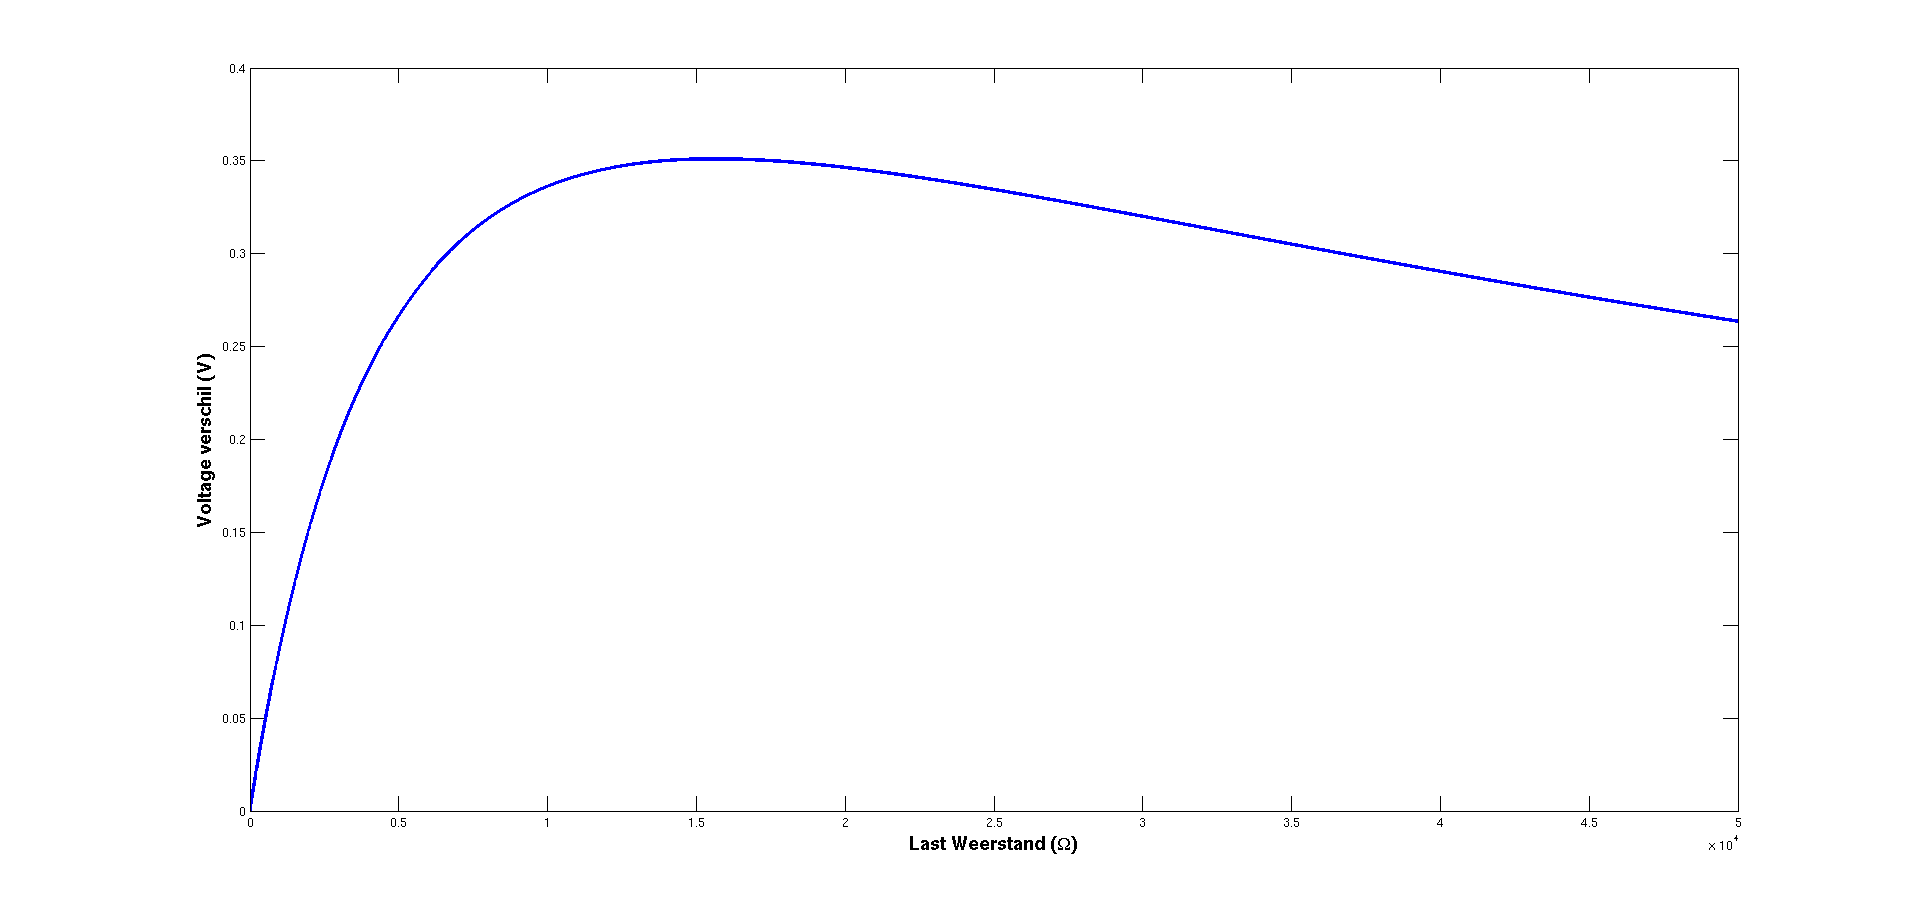
\includegraphics[width=0.8\textwidth]{../fig/hfdst-last-rpiek.png}
  \caption{Timing globalblock}
  \label{fig:rpiek}
\end{figure}



\section{evalueren van de last}
Om verschillende lasten met elkaar te kunnen vergelijken, is het belangrijk om hun eigenschappen allemaal op dezelfde manier te bekomen. Figuur \ref{fig:simsetup} geeft de verschillende aspecten van de gebruikte simulatie setup weer. Het test circuit (Figuur \ref{fig:simcircuit}) stelt een bitlijn voor met een capaciteit van 18fF, wat ruiw weg overeenkomt met een bitlijn met 100 cellen op. Aan deze bitlijn zijn een last, een ontlaad transistor en een memristor weerstand aangesloten. De ontlaad transistor is minimaal gehouden. De memristor weerstand kan de volgende waardes hebben: tussen 5k$\Omega$ en 10k$\Omega$ voor de LRS, tussen de 30k$\Omega$ en 35k$\Omega$ voor de HRS. De nominale waardes voor LRS en HRS zijn 7.5k$\Omega$ en 32.5k$\Omega$. Tijdens monte-carlo analyses worden dan deze nominale waardes als gemiddelde van een gausische distributie genomen met $\sigma = 0.833k\Omega$. Aan deze memristor weerstand hangt een select transistor, die ook minimaal gehouden wordt, en de combinatie van deze word de geheugen cell genoemt. Aan deze geheugen cell hangt nog een selectlijn transistor met een breedte van 500nm. Deze transistor werd bewust groot gemaakt om de totale weerstand in de onderste tak voornamelijk te laten afhangen van de geheugen cell. Aan deze selectlijn werd er ook een weerstand van 18fF aan gehangen, deze doet echtern niet veel aangezie de select transistor altijd aan gelaten wordt. Tenslotte word de voedings spanning altijd op 1V gehouden.\\\\
Figuren \ref{fig:simcontr1} tot \ref{fig:simcontr3} stellen de sequentie van alle controle signalen uit tijden de simulatie. Eerst wordt de bitlijn volledig ontladen (\ref{fig:simcontr1}). Vervolgens is er een interval waar niks gebeurt (\ref{fig:simcontr2}) en tenslotte wordt te last aangesloten en de bitlijn op geladen (\ref{fig:simcontr3}). De simulatie stopt als de bitlijn volledig is opgeladen.\\

\begin{figure}[!ht]
\centering
\subfloat[Test circuit]{ 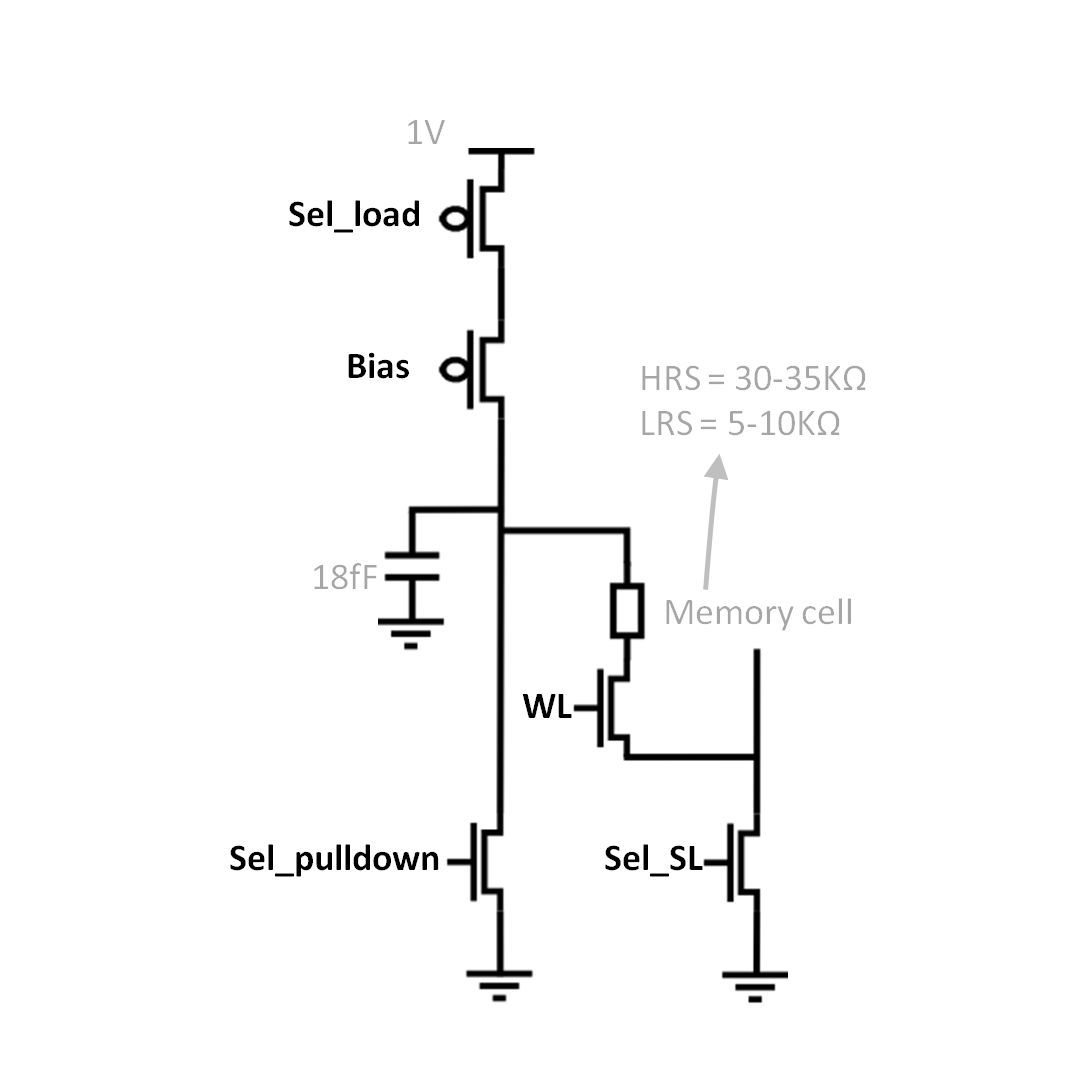
\includegraphics[width=0.45\textwidth] {../fig/hfdst-last-simsetup.png} \label{fig:simcircuit}}
\subfloat[Controle signalen 1]{ 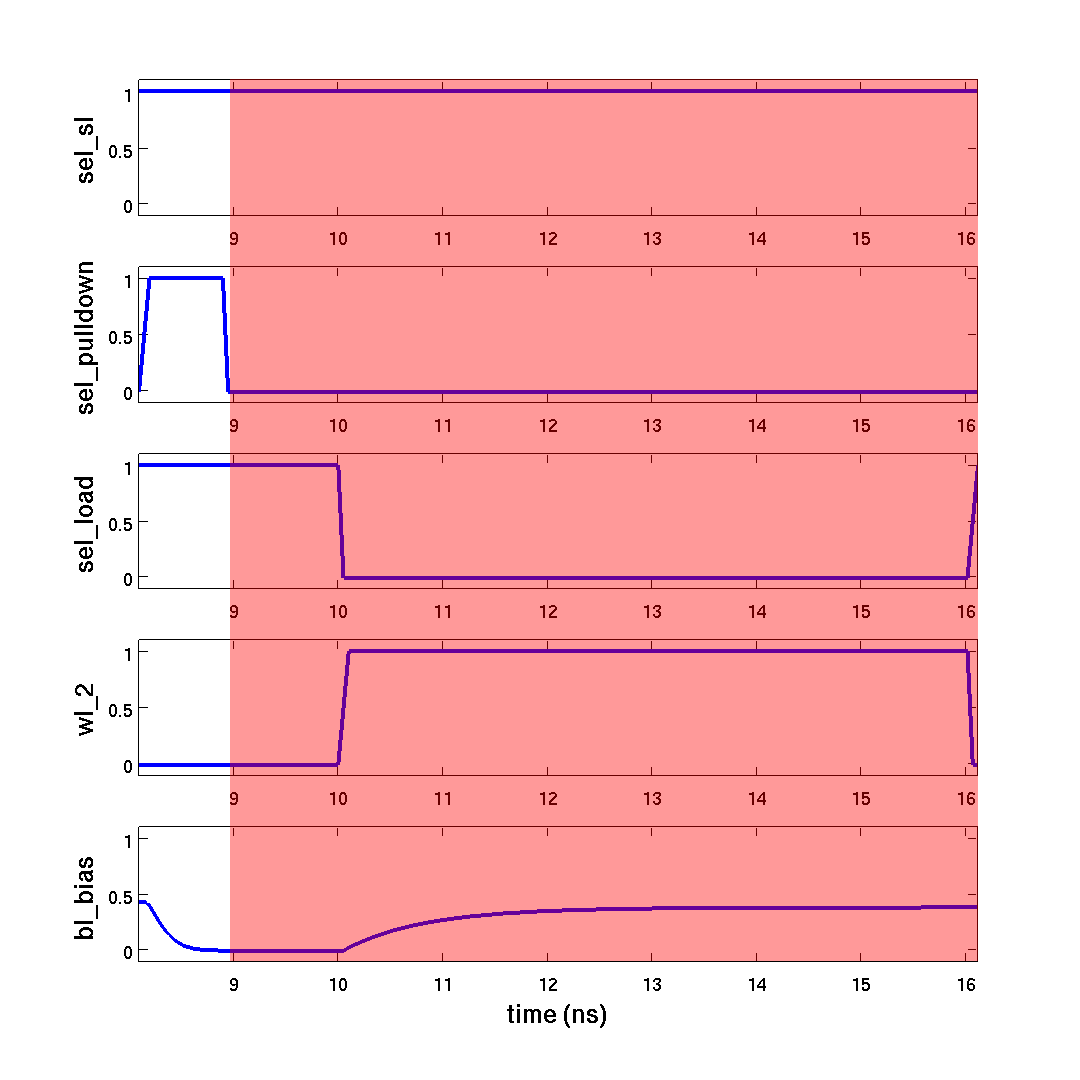
\includegraphics[width=0.45\textwidth] {../fig/hfdst-last-controlsig1.png} \label{fig:simcontr1}}\\
\subfloat[Controle signalen 2]{ 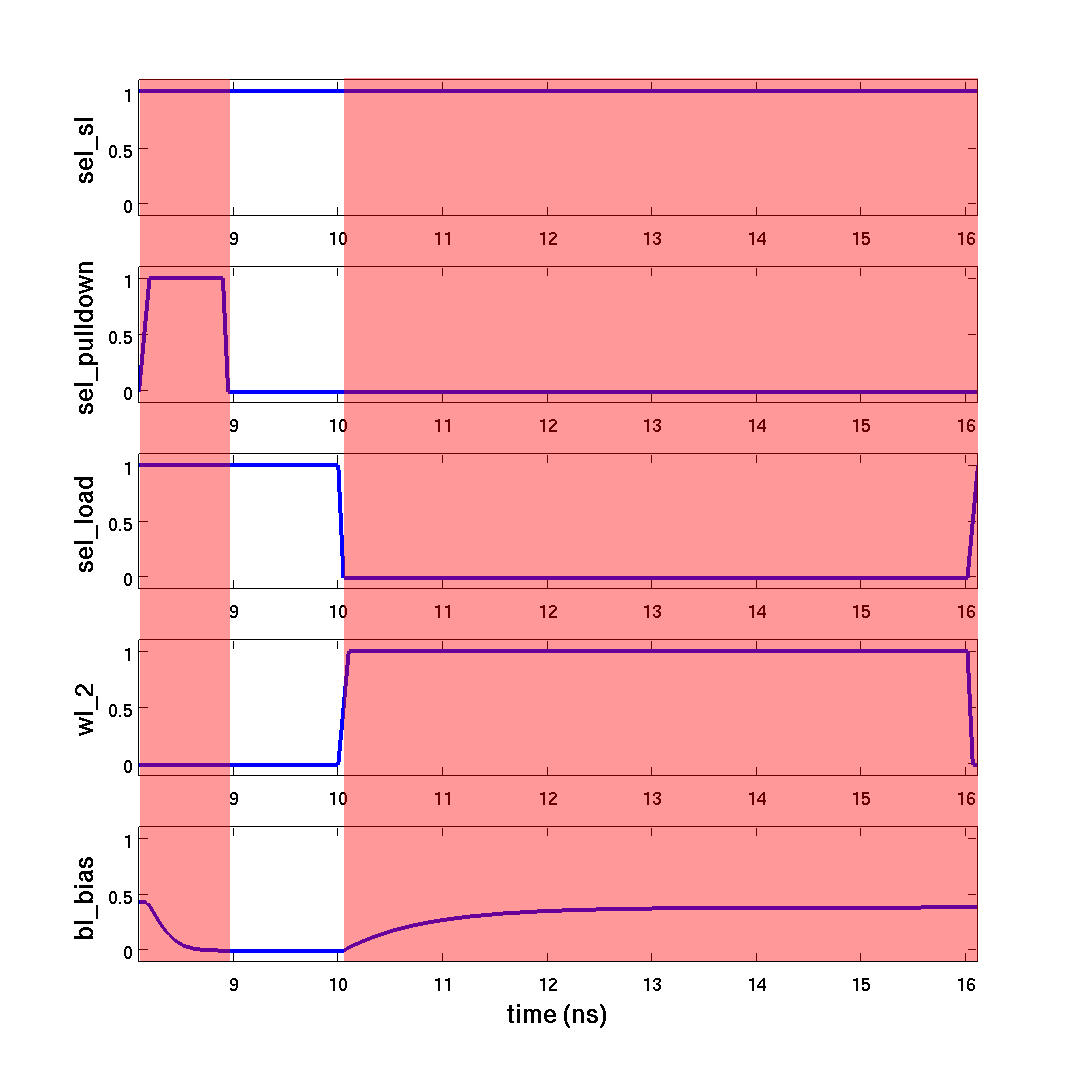
\includegraphics[width=0.45\textwidth] {../fig/hfdst-last-controlsig2.png} \label{fig:simcontr2}}
\subfloat[Controle signalen 3]{ 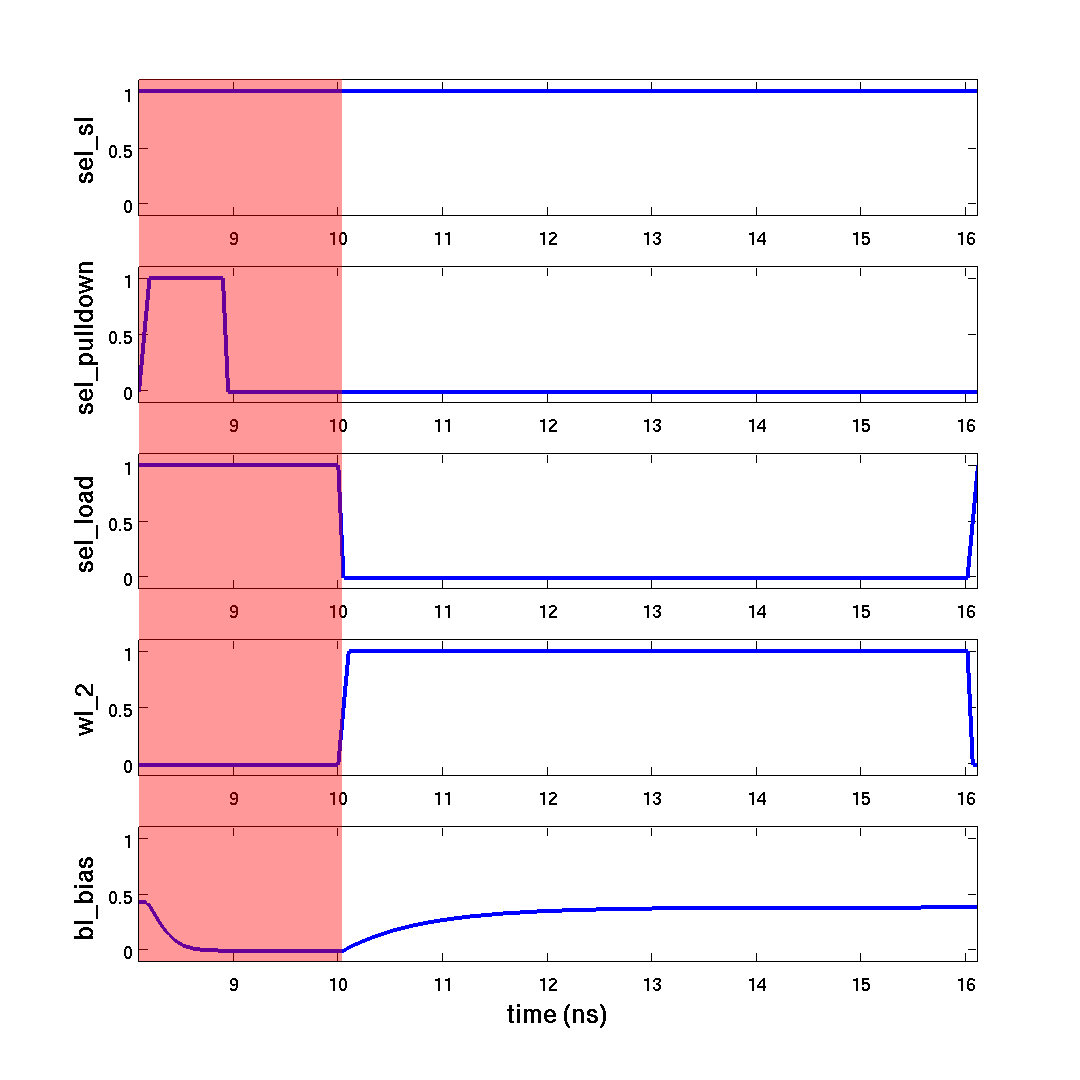
\includegraphics[width=0.45\textwidth] {../fig/hfdst-last-controlsig3.png} \label{fig:simcontr3}}
\caption{Test bench voor de last}\label{fig:simsetup}
\end{figure}

Eens een last gesimuleert is wordt het beoordeelt op het vlak van oppervlakte, bitlijn risetime, nominaal bitlijn voltage verschil en voltage drop over de cell. Het oppervlakte wordt berekend op basis van de lengtes en breetes van de last transistoren. De bitlijn risetime is de tijd dat nodig is om de bitlijn $99\%$ op te laden. Het nominale bitlijn voltage verschil is het verschil in bitlijn voltage tussen een cell in HRS en LRS, wanneer de bitlijn $100\%$ is opgeladen. De bitlijn wordt veronderstelt $100\%$ opgeladen te zijn op het einde van de simulatie en de simulatie tijd word voldoende lang gehouden om dit te garenderen. De spanningsval over de cell is belangrijk opdat de cell in van state wisselt gedurende de leescyclus. Aangezien de cell voorgesteld wordt met een weerstand zal dit natuurlijk nooit gebeuren maar dit is wel belangrijk moest er met echte memristors worden gewerkt. De numerieke waarde van de maximale spannings val over de cell is heel erg afhankelijk van het type memristor. In dit onderzoek wordt er gewerkt met een maximum van 0.5V over de cell.

\section{vergelijking van verschillende types last}
Voor dit onderzoek worden vier mogelijke kandidaten van last vergeleken: de switchload (\ref{fig:switchload}), de biasload (\ref{fig:biasload}), de diodeload (\ref{fig:diodeload}) en de bulkload (\ref{fig:bulkload})\cite{bulkload}. Eerst wordt er een lineare sweep gedaan op verschillende lasten (\ref{sec:linload}), waarbij enkel de breetes en bias spanningen worden gesweepts. De lengtes van de transistoren word minimaal gehouden om er voor te zorgen dat de transistoren binnen de pitch van de bitlijn passen. Eens variabiliteit wordt toegevoegd aan de simulatie onder de vorm van monte-carlo (\ref{sec:varload}), zal echter blijken dat er het verschil in bitlijn voltage te klein is, en zal de lengte van de last transistoren ook moeten worden vergroot (\ref{sec:finaleload}).

\begin{figure}[!ht]
  \centering
  \subfloat[De switch load]{\makebox[.22\textwidth]{ 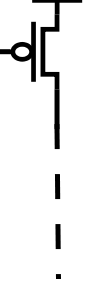
\includegraphics[width=0.12\textwidth] {../fig/hfdst-last-loadtypesswitch.png} \label{fig:switchload}}}
  \subfloat[De bias load]{\makebox[.22\textwidth]{ 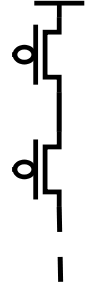
\includegraphics[width=0.12\textwidth] {../fig/hfdst-last-loadtypesbias.png} \label{fig:biasload}}}
  \subfloat[De diode load]{\makebox[.22\textwidth]{ 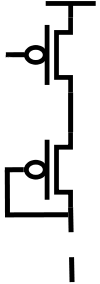
\includegraphics[width=0.12\textwidth] {../fig/hfdst-last-loadtypesdiode.png} \label{fig:diodeload}}}
  \subfloat[De bulk load]{\makebox[.22\textwidth]{ 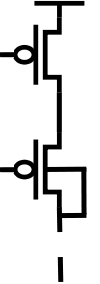
\includegraphics[width=0.12\textwidth] {../fig/hfdst-last-loadtypesbulk.png} \label{fig:bulkload}}}
  \caption{De verschillende types last}
  \label{fig:loads}
\end{figure}

\subsection{Lineaire sweep op de lasten}\label{sec:linload}
\paragraph{}
De switchload bestaat uit \'{e}\'{e}n pmos transistor dit volledig wordt aan of afgesloten. Een lineare sweept met een breedte van de transistor tussen 100nm en 500nm werd gedaan en is geillustreed in figuur \ref{fig:switchloadsim}. Bij het vergroten van de breedte van de transistor zal de weerstand dalen en het verschil tussen de bitlijnen ook. Als we deze last vergelijken men het simpele model uit sectie \ref{sec:simplemodel}, zit de weerstand waarde aan de linker kant van de piek uit figuur \ref{fig:rpiek}. Bij het vergroten van de transistor breedte zal de bitlijn spanning stijgen en de spannings val over de cell dus ook. Verder volgt de risetime ook het simple model uit sectie \ref{sec:simplemodel}, waarbij de risetime daalt bij kleinere weerstands waardes.

\paragraph{}
De biasload, is een last met twee pmos transistoren in serie. Bovenste van de twee wordt als een switch gebruikt en dus volledig aan of af gesloten. De onderste van de twee word op een spanning gebiased. Het voordeel van de biasload is dat men een grotere weerstand kan maken en dus de piek kan bereiken uit figuur \ref{fig:rpiek}. Dit kan men duidelijk zien op de x-assen van figuur \ref{fig:biasloadsim}. Ook hier is de breedtes van de transistoren gesweeepts tussen 100nm en 500nm. De bias spanning is tussen 0V en 0.4V gesweept. Een hogere bias spanning brengt echter geen nuttige bij drage. Door dat te kleinste weerstand dat met deze last te maken is ,binnen deze sweeprange, net iets groter is als deze van de switch load, is de biasload ook iets trager. De oplossingen waarbij dit het geval is, hebben echter een onbruikbaar verschill in bitlijn voltages. De spanningsval over de cell is vergeleken met de switch load heel wat hoger maar voor de meeste oplossingen ligt het nogaltijd onder de limiet van 0.5V.

\paragraph{}
De diode load bestaat ook uit twee transistoren, de bovenste wordt net als bij de biasload als een switch gebruikt. De onderste is als een diode geconnecteerde transistor gekoppelt. Uit de sweept resultaten (figuur \ref{fig:diodeloadsim}) blijkt dat deze last heel snel is maar veel te kleinen bitlijn voltage verschillen heeft om bruikbaar te zijn.

\paragraph{}
De bulkload werd voor gestelt in de paper van Ren et al. \cite{bulkload} als een goede kandidaat omwille van zijn grote uitgangs impedantie. Deze last bestaat uit een switch transistor en een bulk geconnecteerde transistor. Deze bulk geconnecteerde transistor word op 0V gebiast aangezien deze de beste resultaten gaf. De breedtes vab de transistoren zijn gesweept tussen 100nm en 500nm. De resultaten van deze sweep zijn geillustreerd in figuur \ref{fig:bulkloadsim}. In de resultaten kan gezien worden dat deze last zich vergelijkbaar gedraagt als de biaslast. Enkel op het vlak van risetime zijn er oplossingen die beter zijn.

\afterpage{
\begin{figure}
  \centering
  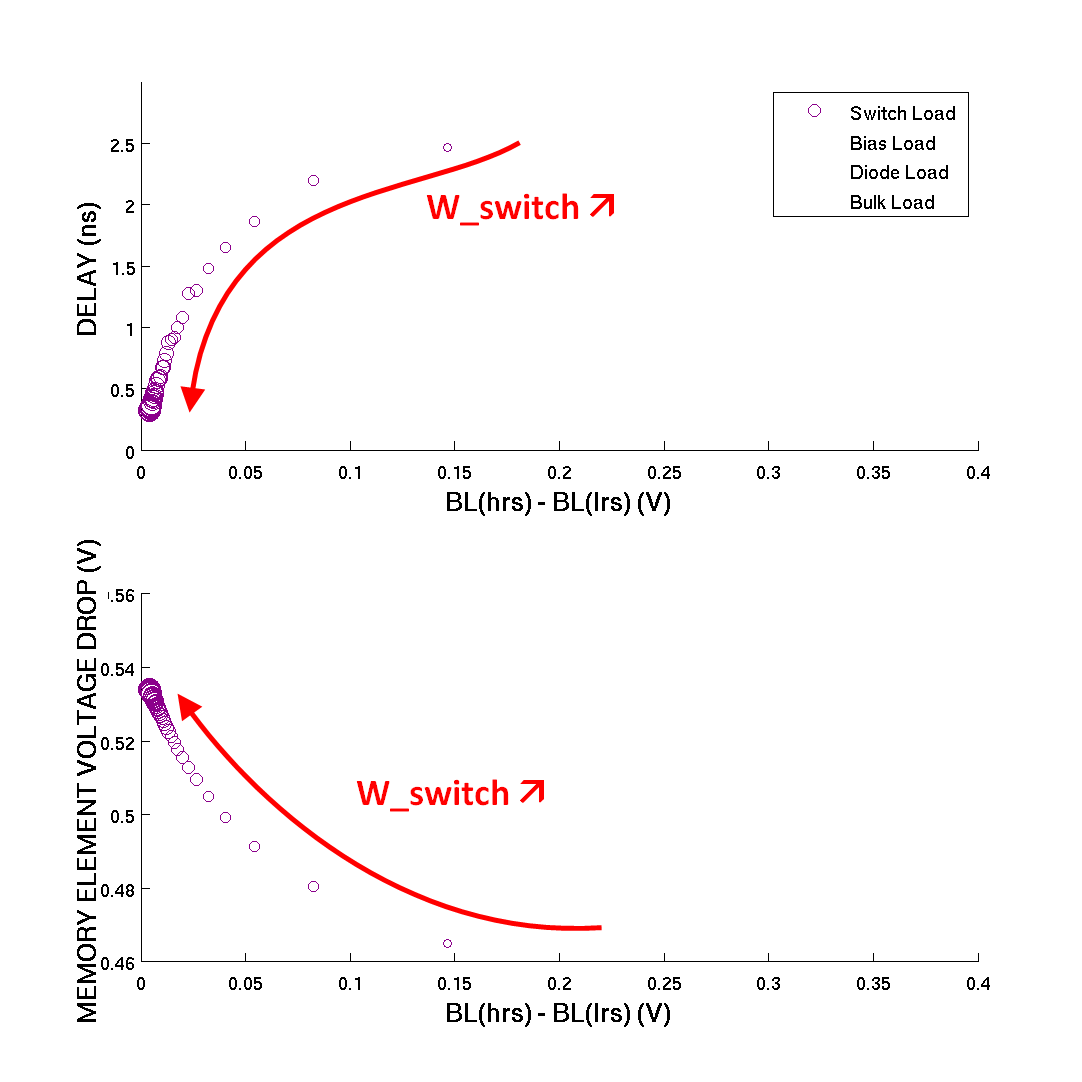
\includegraphics[width=0.67\textwidth]{../fig/hfdst-last-switchload.png}
  \caption{Lineaire sweep van switchload}
  \label{fig:switchloadsim}
 \centering
  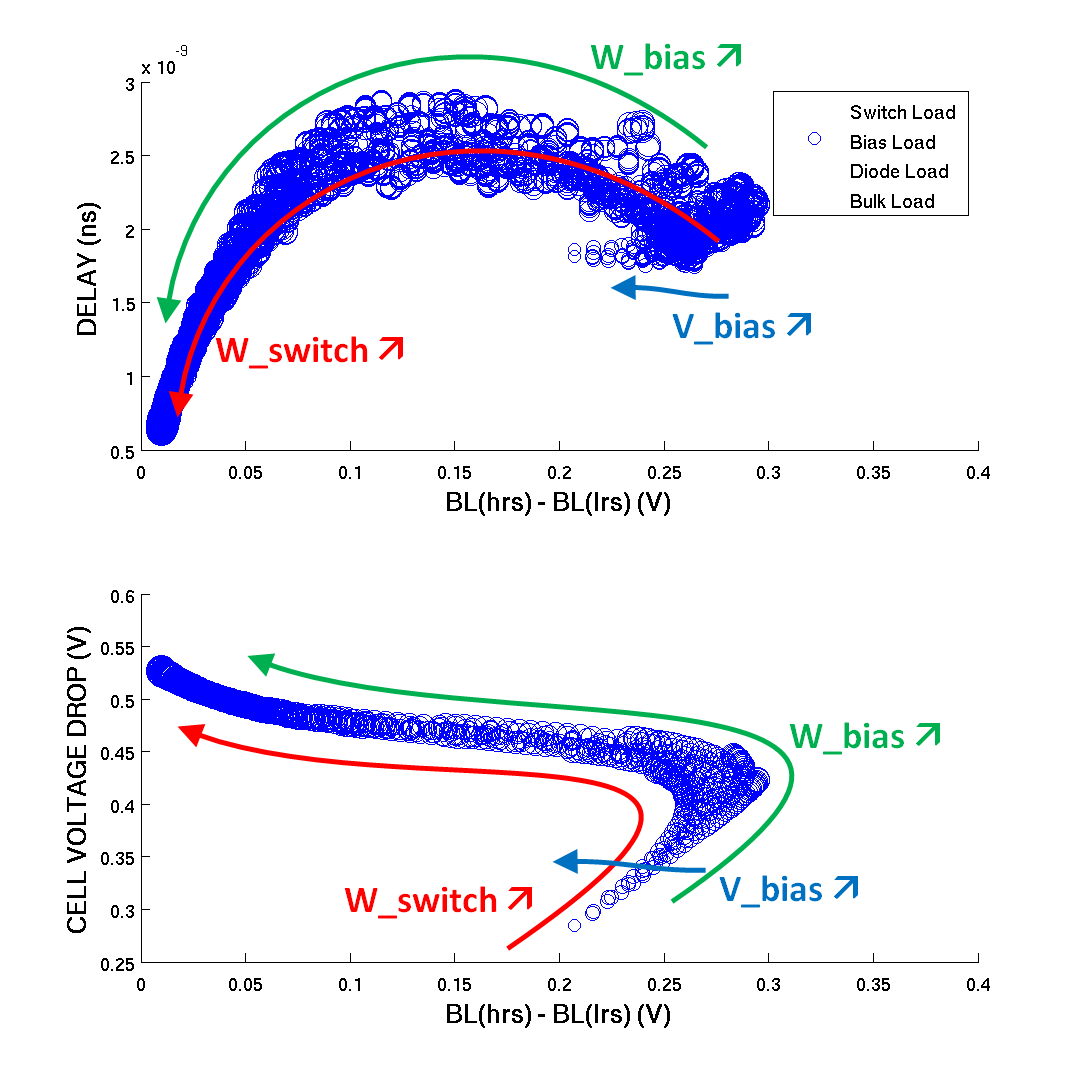
\includegraphics[width=0.67\textwidth]{../fig/hfdst-last-biasload.png}
  \caption{Lineaire sweep van biasload}
  \label{fig:biasloadsim}
\end{figure}
}
\afterpage{
\begin{figure}
  \centering
  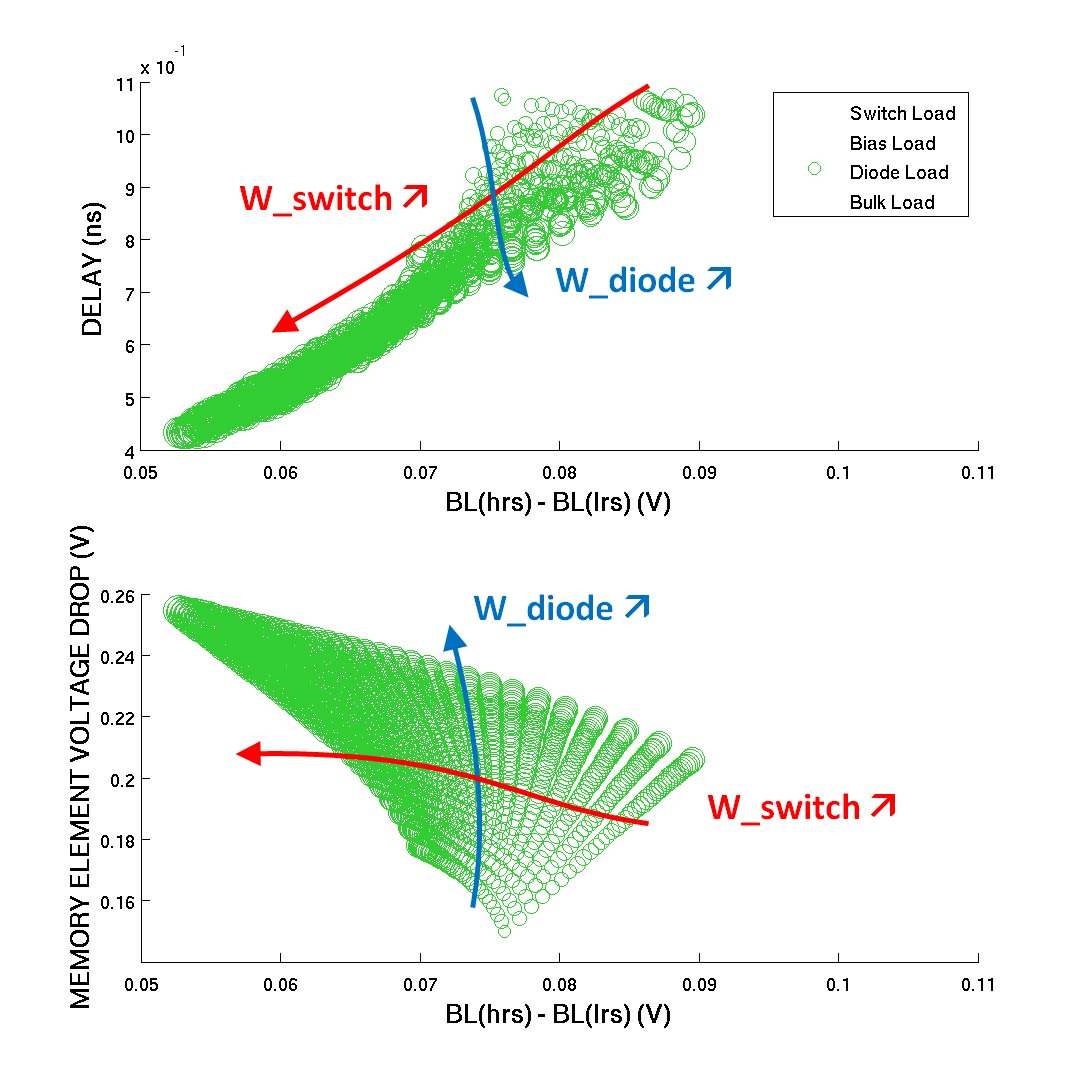
\includegraphics[width=0.67\textwidth]{../fig/hfdst-last-diodeload.png}
  \caption{Lineaire sweep van diodeload}
  \label{fig:diodeloadsim}
  \centering
  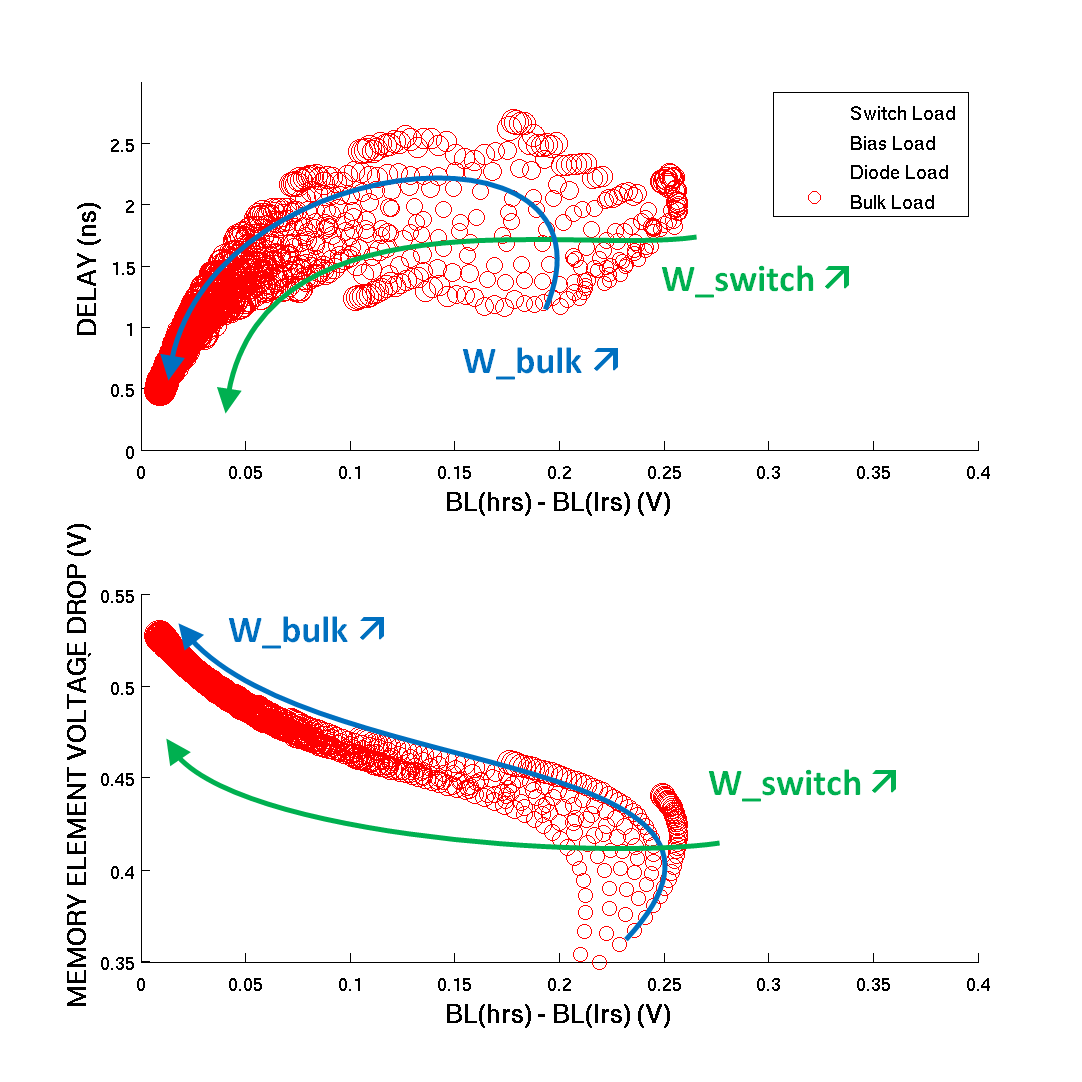
\includegraphics[width=0.67\textwidth]{../fig/hfdst-last-bulkload.png}
  \caption{Lineaire sweep van bulkload}
  \label{fig:bulkloadsim}
\end{figure}
}

\subsection{Het toevoegen van variabiliteit}\label{sec:varload}
Na een selectie te hebben gemaakt van de oplossingen uit de vorige sectie, worden met deze oplossingen nieuwe simulatie gedaan waarbij er variabiliteit is toegevoegt. Deze variabiliteit is toegevoegd op alle transistoren in het test circuit en op de weerstands waarde van de geheugen cellen. Voor de transistoren word er een Pelgrom constante voor vt van $2.5$ gebruikt en voor $\beta$ van $1.2$ gebruikt \cite{ppt:variatie}. Voor de weerstand waarde van de memristors word er een gausische verdeling gebruikt met nominale waardes 7.5k$\Omega$ en 32.5k$\Omega$ en met $\sigma = 0.833k\Omega$. Er worden telkens 500 monte carlo simulaties gedaan per oplossing. Hierna worden de bitlijn voltages van cellen met een HRS en LRS gefit op een gausische distributie. De oplossing met het grootste bitlijn voltage verschil tussen de extrema van HRS en LRS is een biasload met een switch transitor breete van 100nm, een bias transistor breete van 180nm en een bias voltage van 0V. De bitlijn voltage distributie zijn geillustreed op figuur \ref{fig:distbias}. Het voltage verschill tussen de CDF = $0.1\%$ van HRS en CDF = $99.9\%$ van de LRS is 65mV. Dit is niet veel aangezien de distributie van het bitlijn voltage van de referentie cell hier tussen moet passen en er daarna nog marge over moet zijn voor variabiliteit in de senseamplifier. Het aandeel to variabiliteit van beide transistoren in de last is even groot.

\begin{figure}[!h]
  \centering
  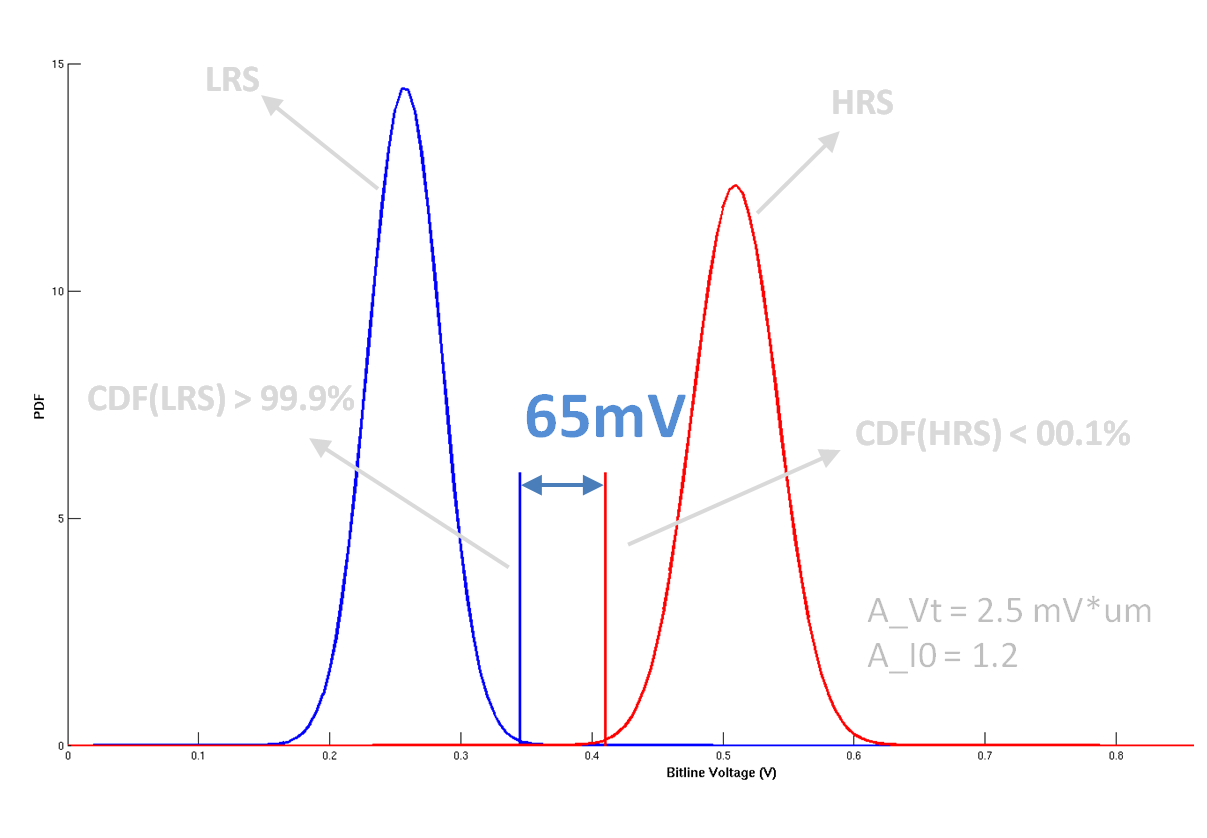
\includegraphics[width=0.67\textwidth]{../fig/hfdst-last-var1.png}
  \caption{Bitlijn voltage distributie voor een biasload}
  \label{fig:distbias}
\end{figure}

Figuur \ref{fig:distref} stelt de distributie van het bitlijn voltage van de referentie cellen voor. Hier bij varieert het aantal referentie cellen van 2 tot 30 en er werd een even groot aantal referentie cell in HRS als LRS gehouden. Zoals gezien kan worden dat met een heel aantal cellen nodig heeft om een distributie breete van 39mV te krijgen. Dit Geeft dan een marge van ongeveer 10mV voor de senseamplifier wat helemaal niet veel is. Daarom word de constraint waarbij de transistor lengte minimaal gehouden word opgeheven in de volgende sectie.

\begin{figure}[!h]
  \centering
  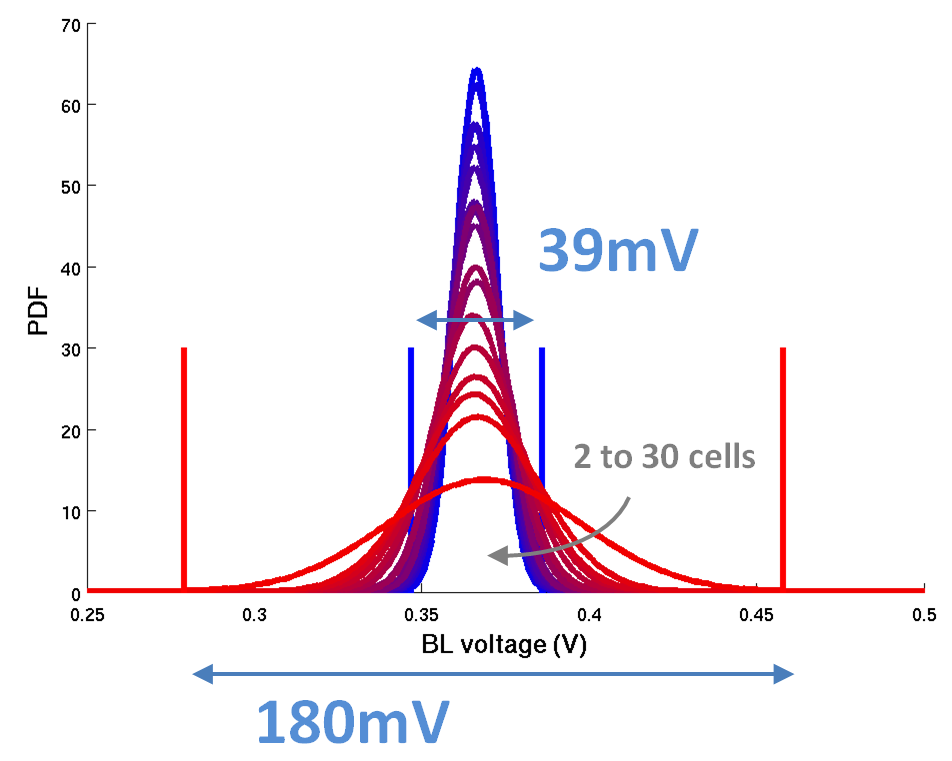
\includegraphics[width=0.67\textwidth]{../fig/hfdst-last-ref.png}
  \caption{Lineaire sweep van switchload}
  \label{fig:distref}
\end{figure}


\subsection{De transistor lengte vergroten}\label{sec:finaleload}
Om de variabiliteit onder controle tehouden moeten de transistoren vergroot worden. Twee opties worden hiervoor overwogen. De eerste is het toevoegen van een derde transistor in serie. Om de zelfde last impedantie te bekomen als voor 2 transisoren in serie, moeten alle drie transistoren een grote breete hebben wat zou betekenen dat ze groter zijn en minder gevoelig voor mismatch. Een aspect waar niet mee rekening word gehouden in die redenering is de toestand waarin deze transistoren zich bevinden. Bij drie transistoren in serie zal de onderste van de drie zich in near tot sub-theashold bevinden. De stroom in het sub-theshold gebied is exponentieel met de gate-source spanning dit levered grote variatie in de stroom voor kleine vt mismatch. Dit fenemeen zien men niet bij 2 transistoren in serie, aangezien de transistoren hier in het lineare gebied zijn. Daarom word er gekozen voor een tweede optie om de mismatch onder controle te houden namelijk het vergroten van de lengte van de transistor. Als men de lengte vergroot, Stijgt de weerstand wat dan weer gecompenseert kan worden door de breedte ook wat te vergroten. Nu men deze constraint laten varen heeft, word er dan ook geopteert om een switchload ipv een bias load te gebruiken.\\
Figuur \ref{fig:length} geeft de resultaten weer van een sweep van verschillende lengtes en breetes voor een switchload. De resultaten worden voor gestelt in functie van $W/L$ wat een indicatie is voor de weerstand van de transistor. In de bovenste figuur kan men duidelijk een maximun zien voor het verschil in bitlijn voltage zoals in sectie \ref{sec:simplemodel} werd voorspelt. Verder wordt opgemerkt dat er best \'{e}\'{e}n van de oplossingen aan de linkerkant van het maximum gekozen wordt aangezien de spannings val over de cell van de oplossingen aan de rechterkant van het maximum te hoog zijn.
\begin{figure}[!ht]
  \centering
  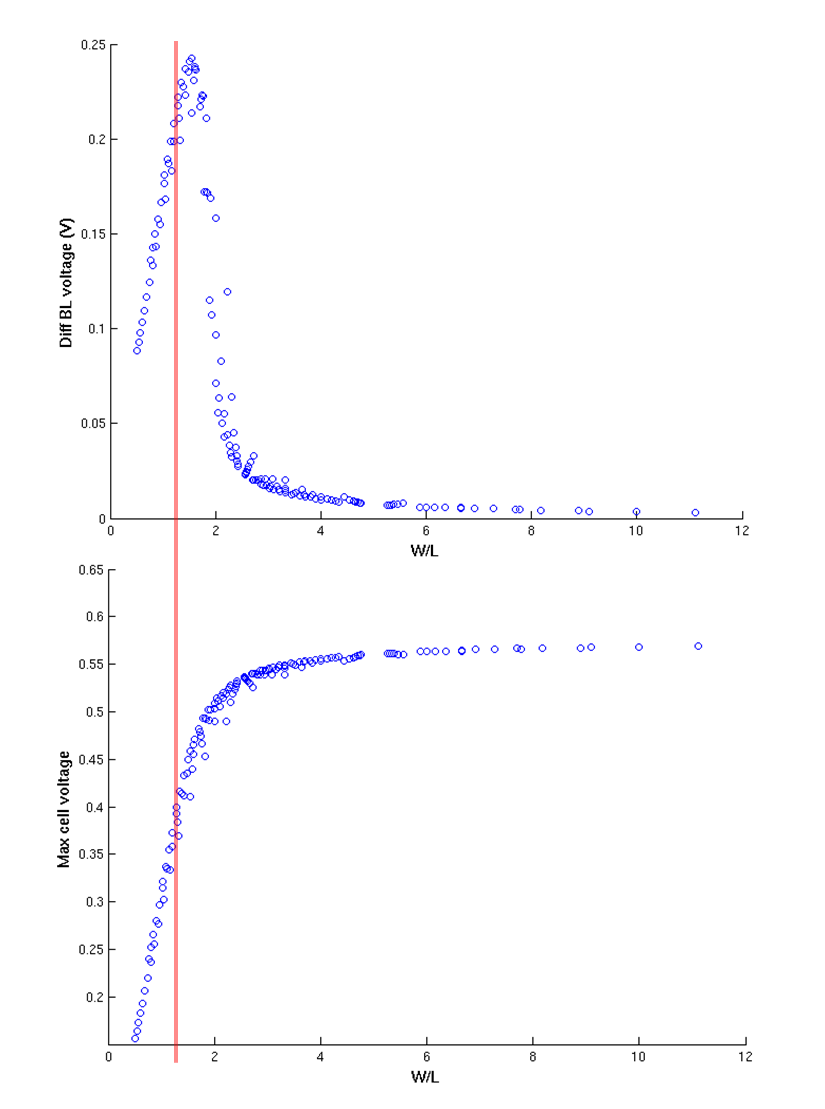
\includegraphics[width=0.80\textwidth]{../fig/hfdst-last-length.png}
  \caption{Verschillende oplossingen voor de switchload met variabele lengtes en breetes}
  \label{fig:length}
\end{figure}

Voor de finale last wordt er geopteert voor een transistor met lengte gelijk aan 198nm en breedte gelijk aan 300nm. Op figuur \ref{fig:length} word deze aangeduid met de rode lijn. Op figuur \ref{fig:distswitch} word de bitlijn voltage distributie van deze last getoont. Het minimale verschil in bitlijn voltage is bijna 200mV. De distributie van bitlijn voltage van de referentie is ook aangegeven op deze figuur. Deze bestaat hier uit 4 referentie cellen waarvan 2 in HRS en 2 in LRS. Opvallend is dat deze referentie niet in het centrum zit tussen de bitlijn voltages van de cellen. Dit kan opgelost worden door een niet gelijk aantal referentie cellen in HRS en LRS te hebben. Aangezien de standaard deviatie op de bitlijn voltages heel wat beter is nu de lengte van de transistoren ook word gesized, kan er gerust gekozen worden voor een last met een kleiner nominaal verschil in bitlijn voltages. Dit kan 2 voordelen met zich mee brengen. Het eerste is dat de spannings val over de cell verlaagt kan worden als met voor een oplossing kiest dan meer links zit van het maximum in figuur \ref{fig:length}. Het Tweede is dat men voor een oplossing kan kiezen waarbij de bitlijn voltages lager zijn wat een energie winst kan opleveren. Ondanks deze voordelen werd er toch geopteert voor de oplossing met het grootste bitlijn voltage verschil.

\begin{figure}[!h]
  \centering
  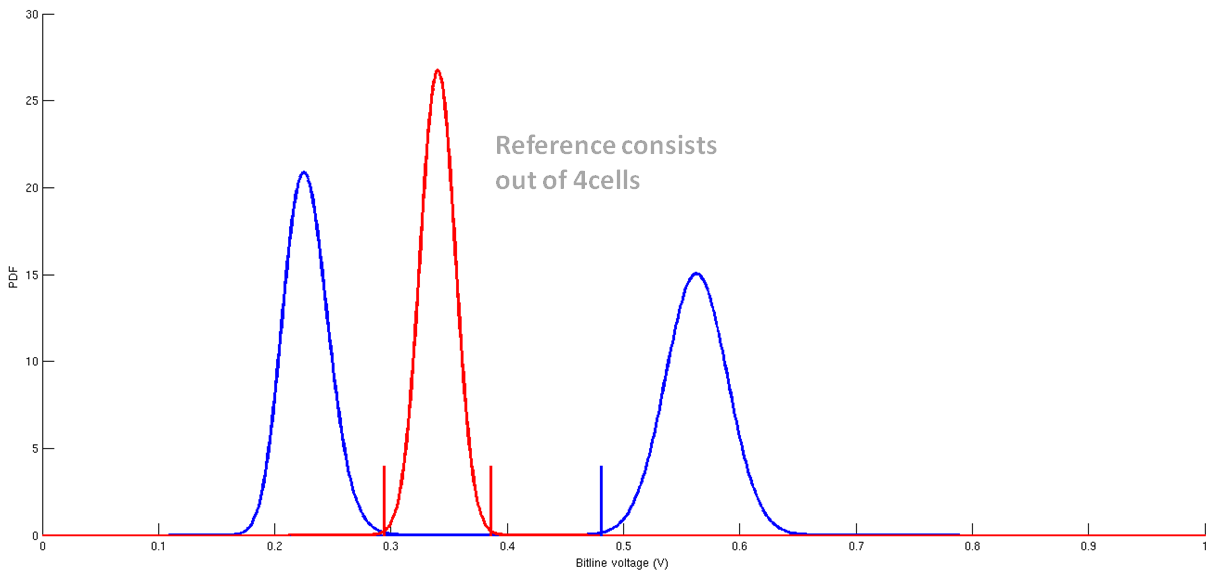
\includegraphics[width=0.67\textwidth]{../fig/hfdst-last-var2.png}
  \caption{Bitlijn voltage distributie voor de finale load}
  \label{fig:distswitch}
\end{figure}